En esta sección se exploran los elementos que intervienen en el desarrollo del software. Se hace un recorrido desde las tecnologías que se utilizarán en el desarrollo, hasta la descripción de los documentos que utilizarán los usuarios del proyecto.
\subsection{Arquitectura}
 
 En este capítulo se presenta la arquitectura y las tecnologías involucradas en el desarrollo de la plataforma. Debido a que en los requisitos del proyecto se contempla que la plataforma quede operativa en la  DTI\footnote{Dirección de Tecnologías e Información de la Universidad Austral de Chile} de la Universidad, el proyecto se tuvo que adaptar a la arquitectura con la que trabaja este departamento.

\subsubsection{Pseudo MVC } \label{PseudoMVC}

El patrón de arquitectura MVC\footnote{Modelo-vista-Controlador} es una filosofía de diseño de aplicaciones que define la organización independiente del Modelo, la Vista  y el Controlador \cite{eje15}. De esta forma, el sistema se divide en tres capas donde el \textbf{modelo}  contiene una representación de los datos que maneja el sistema, es decir, el modelo de datos, la \textbf{ vista}  o interfaz de usuario contiene la información que se envía al cliente y los mecanismos de interacción con éste, y por ultimo, el \textbf{controlador} es el intermediario entre el modelo y la vista, gestionando el flujo de información entre ellos.
\\

Como se ha dicho la arquitectura MVC utiliza la división tradicional en 3 capas (presentación, lógica de negocio y datos) sin embargo la arquitectura de los proyectos de la Universidad no es específicamente  MVC, es más bien una adaptación puesto que no se separa totalmente lo que es vista del controlador, pero si se manejan de forma separada la capa de datos de la capa lógica y la interfaz de usuario, de manera semejante es como trabaja ASP.NET (se explicará en la sección \ref{ASP.NET}) . La arquitectura descrita anteriormente se detallará a continuación.
\\

	\begin{figure}[H]
		\centering
		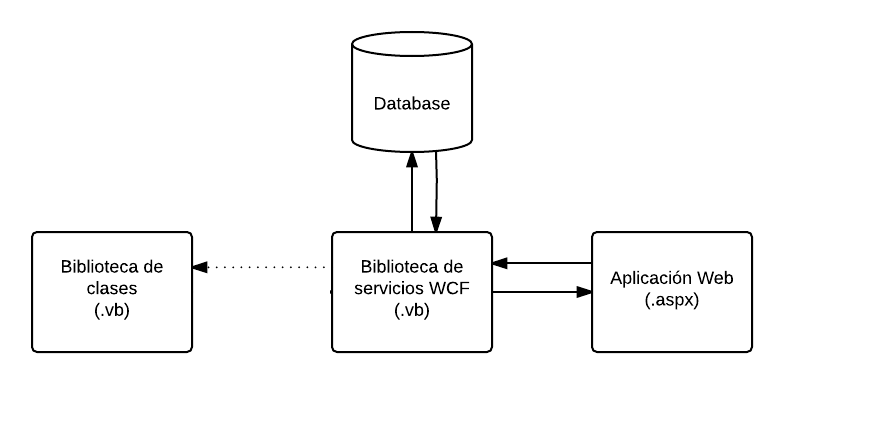
\includegraphics[width=1\textwidth]{images/Capitulo_2/pseudoMVC.png}
		\caption[Arquitectura pseudo MVC Universidad Austral de Chile]{Arquitectura pseudo MVC Universidad Austral de Chile \footnote{}}
		\label{FiguraMVC}
	\end{figure}
	\footnotetext{Elaboración propia.}
	
En la Figura \ref{FiguraMVC} se puede apreciar las 3 capas de esta arquitectua. Esta arquitectura esta compuesta por:
\begin{enumerate}
	\item \textbf{Biblioteca de servicios WCF:} Esta capa responde a eventos, usualmente acciones del usuario, e invoca los procedimientos almacenados del modelo de datos, el cual obtiene la información en la interfaz genérica de Visual Basic: IEnumerable.
	
	\item \textbf{Biblioteca de clases:} Esta capa es la encargada de darle formato a la información obtenida por la biblioteca de servicios WFC, es decir, es la representación específica de la información con la cual el sistema opera.
	
	\item \textbf{Aplicación Web:} Esta capa es la encargada de interactuar con el usuario, en ella se muestra toda la información ordenada y entendible por el usuario, sin embargo no solo posee código front-end (html, css, JavaScript, etc), si no también métodos que se comunican con los servicios WCF. Es por ello que la vista  no esta del todo separada de las reglas de negocio.
\end{enumerate}

Si bien estas tres capas son importantes, la capa  que se explicará a continuación es la primera, es decir, la biblioteca de servicios WCF, puesto que las bibliotecas de clase no son mas que un conjunto de clases que definen las entidades de la base de datos, y la aplicación web es  el  conjunto de archivos(aspx, js, css, jpg, etc) que permiten al usuario realizar acciones sobre el Sitio Web.
\\

\myparagraph{Biblioteca de servicios WCF}

Hasta el momento, el servicio de mensajería entre aplicaciones se realizaba mediante los protocolos COM, DCOM o MSQM, que obligaba a los programadores a ceñirse no sólo a una forma de programación concreta, sino que también estaba atada a la plataforma y al lenguaje de programación. Los servicios web surgen con el propósito de cambiar esta filosofía, permitiendo hacer la comunicación independiente de lenguaje de programación y plataforma gracias a la creación de estándares de comunicación \cite{WCF15}.
\\

Hoy en día  existen diversos protocolos sobre los que los servicios web pueden operar, sin embargo  son dos los protocolos mas usados por los servicios web:
\begin{itemize}
	\item \textbf{SOAP:} \textit{Simple Object Access Protocol.} Utiliza XML como lenguaje de codificación, y su principal ventaja es que puede ser transmitido por cualquier capa de transporte (HTTP, TCP/IP, SMTP, etc).

	
	\item \textbf{REST:} \textit{Representational State Transfer.} A diferencia del protocolo  aterior, REST solo puede utilizar la capa de transporte HTTP, sin embargo su filosofía se  basa en la ausencia de estado y la “equivalencia” entre los cuatro verbos que pueden utilizarse en el protocolo HTTP y las cuatro operaciones CRUD (Create, Read, Update, Delete) básicas que pueden realizarse sobre una fuente de datos. 
\end{itemize}



 
Windows Communication Foundation (WCF)  es un marco de trabajo para la creación de aplicaciones orientadas a servicios, su principal objetivo  es el de unificar las comunicaciones, es decir las aplicaciones que utilicen WCF pueden  implementar varios protocolos de servicio web, por lo que permite que el código sea independiente del protocolo que se utilice.
\\

WCF logra su independencia mediante la separación entre operaciones y datos, en otras palabras, un servicio web WCF establece un contrato a través de una interfaz y una clase es la encargada de implementarla. De este modo, un servicio WCF, se compondrá de los siguientes componentes:

\begin{itemize}
	
	\item \textbf{Contrato de servicio (ServiceContract):} expone una operación que el servicio web es capaz de ejecutar. Corresponde a una interfaz.
	
	\item \textbf{ Contrato de datos (DataContract):} implementa un tipo de dato que el servicio web será capaz de manejar. Generalmente, será el tipo de dato que manejará el contrato de servicio.
	
	\item \textbf{Implementación del servicio:} implementará la interfaz correspondiente al contrato de servicio, haciendo uso del contrato de datos para intercambiar la información.
	
\end{itemize}
 
 Los anteriores componentes de un servicio WCF se pueden apreciar gráficamente en la Figura \ref{FiguraWCF}.
 
 	\begin{figure}[H]
 		\centering
 		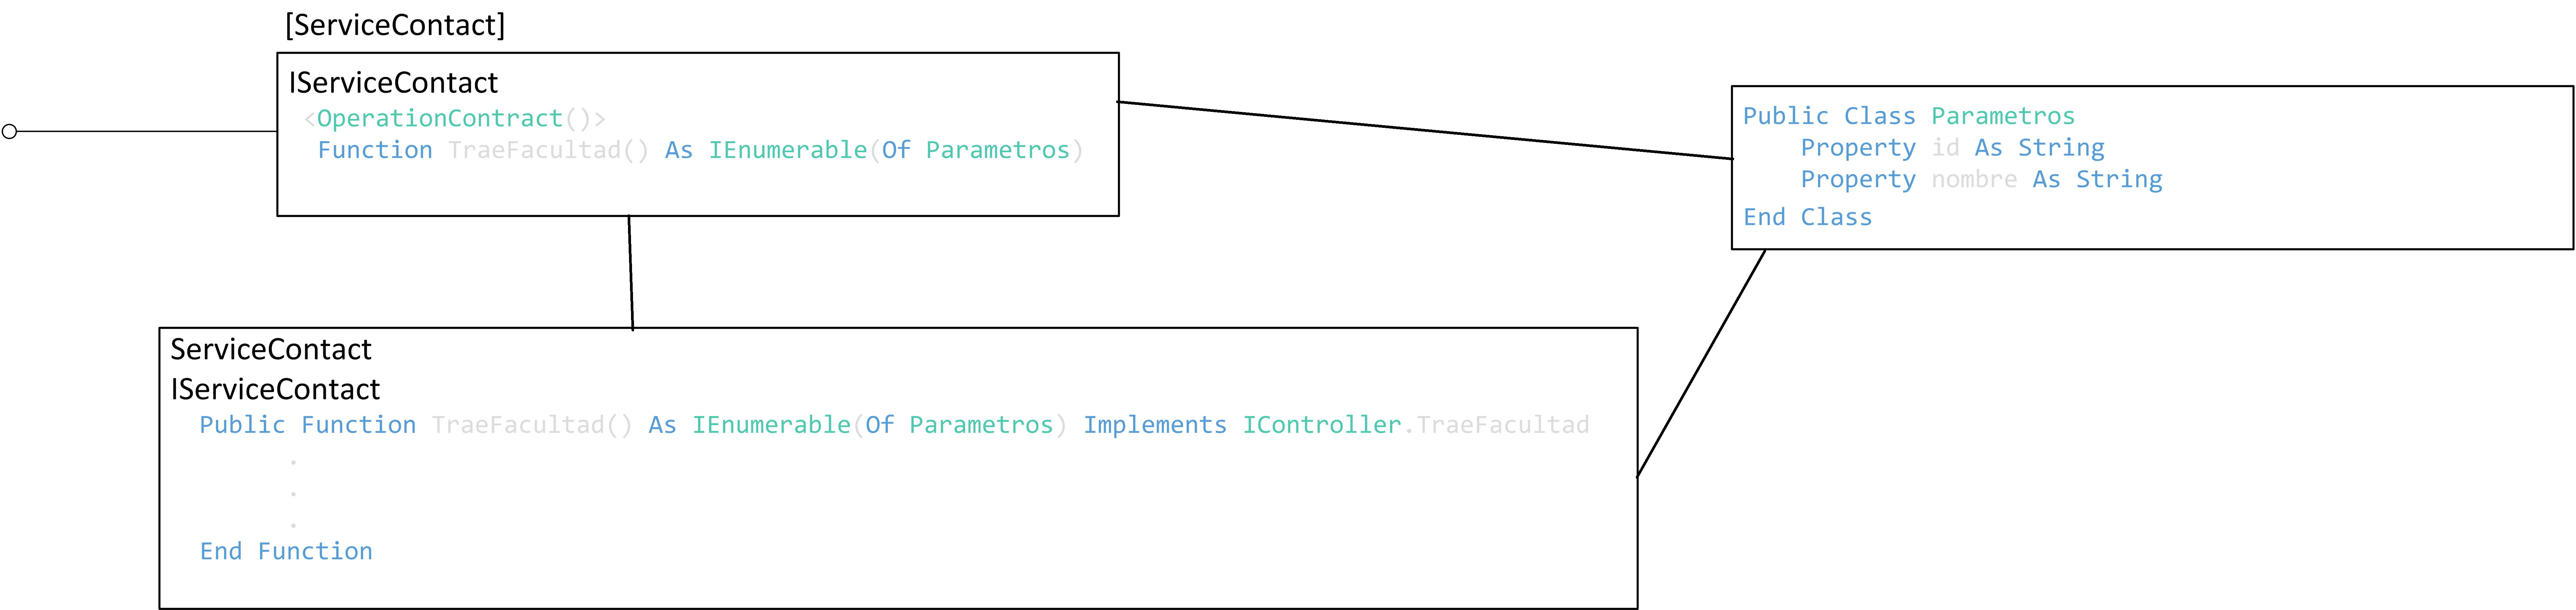
\includegraphics[width=1\textwidth]{images/Capitulo_2/WFC.png}
 		\caption[Diagrama de componentes de un servicio WCF]{Diagrama de componentes de un servicio WCF \footnote{}}
 		\label{FiguraWCF}
 	\end{figure}
 	\footnotetext{Elaboración propia.}

Podemos condensar lo dicho hasta aquí, que el framework que utiliza la Universidad Austral de Chile es una forma distinta de crear aplicaciones web, si bien, se identifican claramente  la división tradicional en 3 capas (presentación, lógica de negocio y datos) no es la misma que propone el patrón MVC. En particular, en esta arquitectura  la capa \textbf{Controller} no tendría una clara correspondencia en la estructura clásica, si no que es  una mezcla de la interfaz gráfica y la lógica del negocio.

\subsection{Tecnologías para el desarrollo de la plataforma} \label{Tecnologias}

A continuación se presentan las distintas tecnologías utilizadas para el desarrollo de la plataforma en sus respectivas capas.
\subsubsection{Front-end}

Esta capa es la parte del software que interactúa con el o los usuarios, en ésta  se encuentran todas las tecnologías que corren del lado del cliente, es decir, todas aquellas tecnologías que corren del lado del navegador web. Es por ello que es de vital importancia de que el front-end sea capaz de entregar  al usuario todas las herramientas necesarias para que éste pueda realizar una correcta interacción con el sistema. Entre las tecnologías usadas en esta capa se encuentran las habituales en el desarrollo Web, tales como HTML, CSS y JavaScript junto con otras que se describirán a continuación.

\myparagraph{JQuery}

JQuery es una librería JavaScript rápida, liviana y con amplias funcionalidades. Hace mucho más simple tareas como recorrer y manipular un documento HTML, manejar eventos, animaciones, e interacciones Ajax	\footnote{Ajax: Asynchronous JavaScript And XML} por medio de una API fácil de usar que funciona a través de múltiples navegadores. Con una combinación de versatilidad y capacidad de ampliación, esta librería busca cambiar la forma en que las personas escriben JavaScript \cite{JQu15}.
\\

Si bien existen otras librerías de JavaScript (Prototype, MoonTools, entre otros). Se decidió usar JQuery en el proyecto por los siguientes motivos:
\begin{itemize}
	\item Es de uso general, por lo que posee una comunidad activa y una extensa documentación.
	\item Posee una amplia variedad de complementos que facilitan el desarrollo.
	\item Es modular.
	\item Es compatible con todos los navegadores existentes.
\end{itemize}


\myparagraph{Alertify}

Alertify es un script escrito con Jquery, el cual nos permite utilizar los siguientes elementos Javascript personalizados: alert(), confirm() y prompt(). Además también nos permite utilizar sus notificaciones, las cuales son muy agradables y sencillas de utilizar y modificar\cite{ALE15}.
\\

Alertify ha sido construido para personalizar nuestras alertas y notificaciones, de esta manera el front-end de la plataforma es mas amigable al usuario y esto permite un mejor entendimiento de los eventos que se realizan en tiempo de ejecución. Además es un plugin multi-idioma y posee responsive-design \footnote{ \textbf{ Responsive Design} es un nuevo paradigma del desarrollo web. Permite adaptar cada sitio a los diferentes formatos de dispositivos de acceso; smartphones, tabletas, portátiles, etc.}
\\

A pesar de que la mayoría de los plugins de notificaciones presentan inconvenientes al momento de implementar con vb.net, se decidió usar un sistema de alertas principalmente para facilitar la visualización de todos los eventos que ocurren en el sistema, y Alertify fue el plugin que menos problemas presentó al momento de la integración con vb.NET.


\myparagraph{Bootstrap}

Bootstrap fue creado a mediados del 2010 por un diseñador y un desarrollador de la red social Twitter, es un proyecto de código abierto, y es uno de los frameworks de front-end más populares en el mundo. Sirvió como guía de estilo para el desarrollo de herramientas internas en la empresa durante más de un año antes de su lanzamiento público, y continua haciéndolo hoy en día\cite{boo15}.
\\

El uso de un framework hace posible que el desarrollo del front-end sea: Fácil, ya que la mayoría de los framework posee una curva de aprendizaje baja, es decir, poseen una gran eficiencia en el  aprendizaje, lo que permite dominar la mayoría de los componentes en un tiempo reducido; Optimizado para dispositivos móviles, puesto que bootstrap posee todas las reglas CSS necesarias para hacer que los sitios se  adapten dinámicamente a la gran mayoría de pantallas y resoluciones existentes en el mercado.


\myparagraph{Template Metis}

Un template es un conjunto de archivos que determinan la estructura y el aspecto visual de un sitio web, y tiene como ventaja principal disminuir tiempos y costos de desarrollo \cite{gli15}. 
\\

El uso de un template disminuye el tiempo de desarrollo de un diseño web, por lo que el alumno tesista se puede centrar en la funcionalidad del sistema que es lo principal."Metis es una  template de administración gratuito basado en Twitter Bootstrap 3.x"\cite{git15}, fue diseñado por un usuario de gitHub y lo puso a disposición para que cualquier usuario lo pueda utilizar.

\myparagraph{Parsley}

 Parsley es una librería de validación de formularios, le ayuda a proporcionar a los usuarios información sobre su envío de formulario antes de enviarlo al servidor \cite{PAR15}. Fue creado por Guillaume Potier y actualmente es sustentado por Marc-André. 
\\

El uso de esta librería se sustenta en el hecho de que notificar los errores de forma inmediata  mejora la satisfacción del usuario con la aplicación y ayuda a reducir la carga de procesamiento innecesario en el servidor.

\subsubsection{Back-end}

El back-end es el área que se dedica a la parte lógica de un sitio web, es el encargado de que todo funcione como debería, el back-end no es visible para el usuario ya que no se trata de diseño, o elementos gráficos, se trata de programar las funciones que tendrá un sitio.

\myparagraph{Microsoft SQL Server 2008}

Microsoft SQL Server 2008 Express es un sistema de administración de datos eficaz y confiable que ofrece un variado conjunto de características, protección de datos y rendimiento para clientes de aplicaciones incrustadas, aplicaciones web ligeras y almacenes de datos locales \cite{mic15}.
\\



Microsoft Sql Server  esta catalogado como  una herramienta fácil de instalar, usar y administrar, por lo que muchas organizaciones hacen uso de sus servicios, tales como  Itaú, Samsung, Marcopolo, entre otras grandes compañías.
\\


Para un manejo adecuado de la base de datos se utilizará SQL Server Management Studio(SSMS), que es `` un entorno integrado para obtener acceso, configurar, administrar y desarrollar todos los componentes de SQL Server.SSMS combina un amplio grupo de herramientas gráficas con una serie de editores de script enriquecidos que permiten a desarrolladores y administradores de todos los niveles obtener acceso SQL Server" \cite{mic15}.







\myparagraph{ASP.NET} \label{ASP.NET}

ASP.NET es una plataforma web que proporciona todos los servicios necesarios para compilar aplicaciones web empresariales basadas en servidor. ASP.NET está compilado en .NET Framework, por lo que todas las características de .NET Framework están disponibles en las aplicaciones ASP.NET. Las aplicaciones se pueden escribir en cualquier lenguaje que sea compatible con Common Language Runtime (CLR), incluido Visual Basic y C\# \cite{inf15}. 
\\

ASP.NET  introduce el concepto del code-behind en el desarollo web, el cual separa el código de la interfaz de usuario, es decir,  todo lo relacionado con la Interfaz de usuario se maneja en el archivo .aspx y el control de los eventos en un archivo separado .vb (Visual Basic).Con ello se facilita la programación de aplicaciones en múltiples capas, lo que en definitiva se traduce en la total separación entre lo que el usuario ve y lo que la base de datos tiene almacenado.La ventaja del modelo  code-behind  es que no se lee secuencialmente sino que se compila, lo que incrementa de velocidad de respuesta del servidor. Además, al compilarse, el incremento en seguridad y fortaleza es muy grande. 
\\

Otro aspecto a tener en cuenta de ASP.NET es que sirve tanto para Webs sencillas como para grandes aplicaciones, ya que la orientación a objetos y la naturaleza compilada permite que la programación de sitios web sea sencilla.

\subsubsection{Herramientas Anexas}

	Esta sección contiene información detallada acerca de todas las herramientas  que  facilitaron la creación e implementación del proyecto. No se clasifican ni en Front-End ni en Back-End dado que son herramientas de gestión y de corrección de errores, por lo que el software final no las contendrá.
	\myparagraph{GitHub}
	
	 El control de versiones es un sistema que registra los cambios realizados sobre un archivo o conjunto de archivos a lo largo del tiempo, de modo que puedas recuperar versiones específicas más adelante \cite{git15}, dicho de otra manera, un control de versiones permite guardar “fotografías” del estado de un proyecto en ese instante del tiempo, dando la capacidad de restaurar ese estado en cualquier momento. Esto ayuda a trabajar en un proyecto y si sale algo mal se puede volver atrás, a algún punto en donde todo funcionaba correctamente.
	 \\
	 
	 A pesar de que existen diversos sistemas de control de versiones y diversos métodos  de control de versiones control de versiones locales, control de versiones centralizados y control de versiones distribuidos), se escogió GitHub por las siguientes razones.
	 
	 \begin{enumerate}
	 	\item Sistema distribuido: en el que todos los nodos manejan la información en su totalidad y por lo tanto pueden actuar de cliente o servidor en cualquier momento, es decir, se elimina el concepto de “centralizado”.
	 	
	 	\item Trabajo en local: Al tener una copia del proyecto se pueden hacer commits de forma local, una vez que se tenga conexión a internet se realiza el commits al servidor.
	 	
	 	\item Fotografías, no diferencias: Cuando un archivo no cambia, en lugar de guardar la misma “fotografía” varias veces, guarda una referencia a esa “fotografía”. De esta forma se optimizan los recursos del sistema. 
	 	
	 \end{enumerate}
	 
	 Es necesario recalcar que en  el proyecto de titulación solo existe un programador, por lo que  no es necesario que el gestor de versiones sea centralizado, de manera que  GitHub cumple con lo que se necesita para el desarrollo del software, el cual es guardar las versiones en caso de cometer algún error en el futuro.
	 
	\myparagraph{Firebug}
	
	Muchas veces es difícil saber qué errores se cometen en el desarrollo y cómo solucionarlos, pero con ayuda de algunos programas, se puede reducir el tiempo que se pierde en la búsqueda de los problemas o errores cometidos. 
	\\

	Si bien uno de los requisitos no funcionales es que la aplicación funcione en los 3 navegadores mas usado a nivel mundial, el desarrollo y las pruebas se  hicieron bajo el navegador Firefox, por lo que se tenia que tener alguna herramienta compatible con este navegador para poder encontrar los errores de manera fácil.
	\\
	
	Firebug es un plugin de Firefox que nos brinda un paquete de utilidades para el desarrollo de páginas y aplicaciones Web. Nos permite debugear, monitorizar y modificar el CSS, HTML y JavaScript en tiempo de ejecución \cite{moz15}. Dicho de otra manera, Firebug no solo debuguea los errores, si no que también el usuario puede monitoriar todas las  peticiones de red que se realizan, entre las mas utilizadas: Petición GET, Petición POST.
	
	

\subsection{Tipos de documentos}



Como se mencionó en la Sección \ref{intro}, existen distintos  tipos de documentos que  dan origen a  alguna modificación curricular, los cuales se nombrarán a continuación.

\begin{itemize}
	\item Comunicación Interna.
	\item Correos electrónicos.
	\item  Resolución (Vicerrectoría Académica, Dirección de Estudios de Pregrado, Secretaria General).
	\item Decretos.
	\item Programas de asignaturas.
\end{itemize}




